\newpage

\section{Ход работы}

\subsection{Калибровочный график зависмости}

Используя милливеберметр, будем изменять значение $I_M$ на генераторе. Таким образом, найдём зависимость значения $B$ от $I_M$.

% Please add the following required packages to your document preamble:
% \usepackage[table,xcdraw]{xcolor}
% Beamer presentation requires \usepackage{colortbl} instead of \usepackage[table,xcdraw]{xcolor}
\begin{table}[H]
\centering
\caption{Калибровка электромагнита}
\label{t1}
\begin{tabular}{|c|c|c|}
\hline
\rowcolor[HTML]{A9D08E} 
B, мТ & I, мА & $\sigma_{B}$, мТ \\ \hline
18.0  & 0    & 0.9              \\ \hline
127   & 0.12 & 6                \\ \hline
249   & 0.24 & 12               \\ \hline
359   & 0.36 & 18               \\ \hline
470   & 0.49 & 20               \\ \hline
590   & 0.61 & 30               \\ \hline
690   & 0.73 & 30               \\ \hline
880   & 0.96 & 40               \\ \hline
1090  & 1.21 & 50               \\ \hline
\end{tabular}
\end{table}\begin{figure}[H]
    \centering
    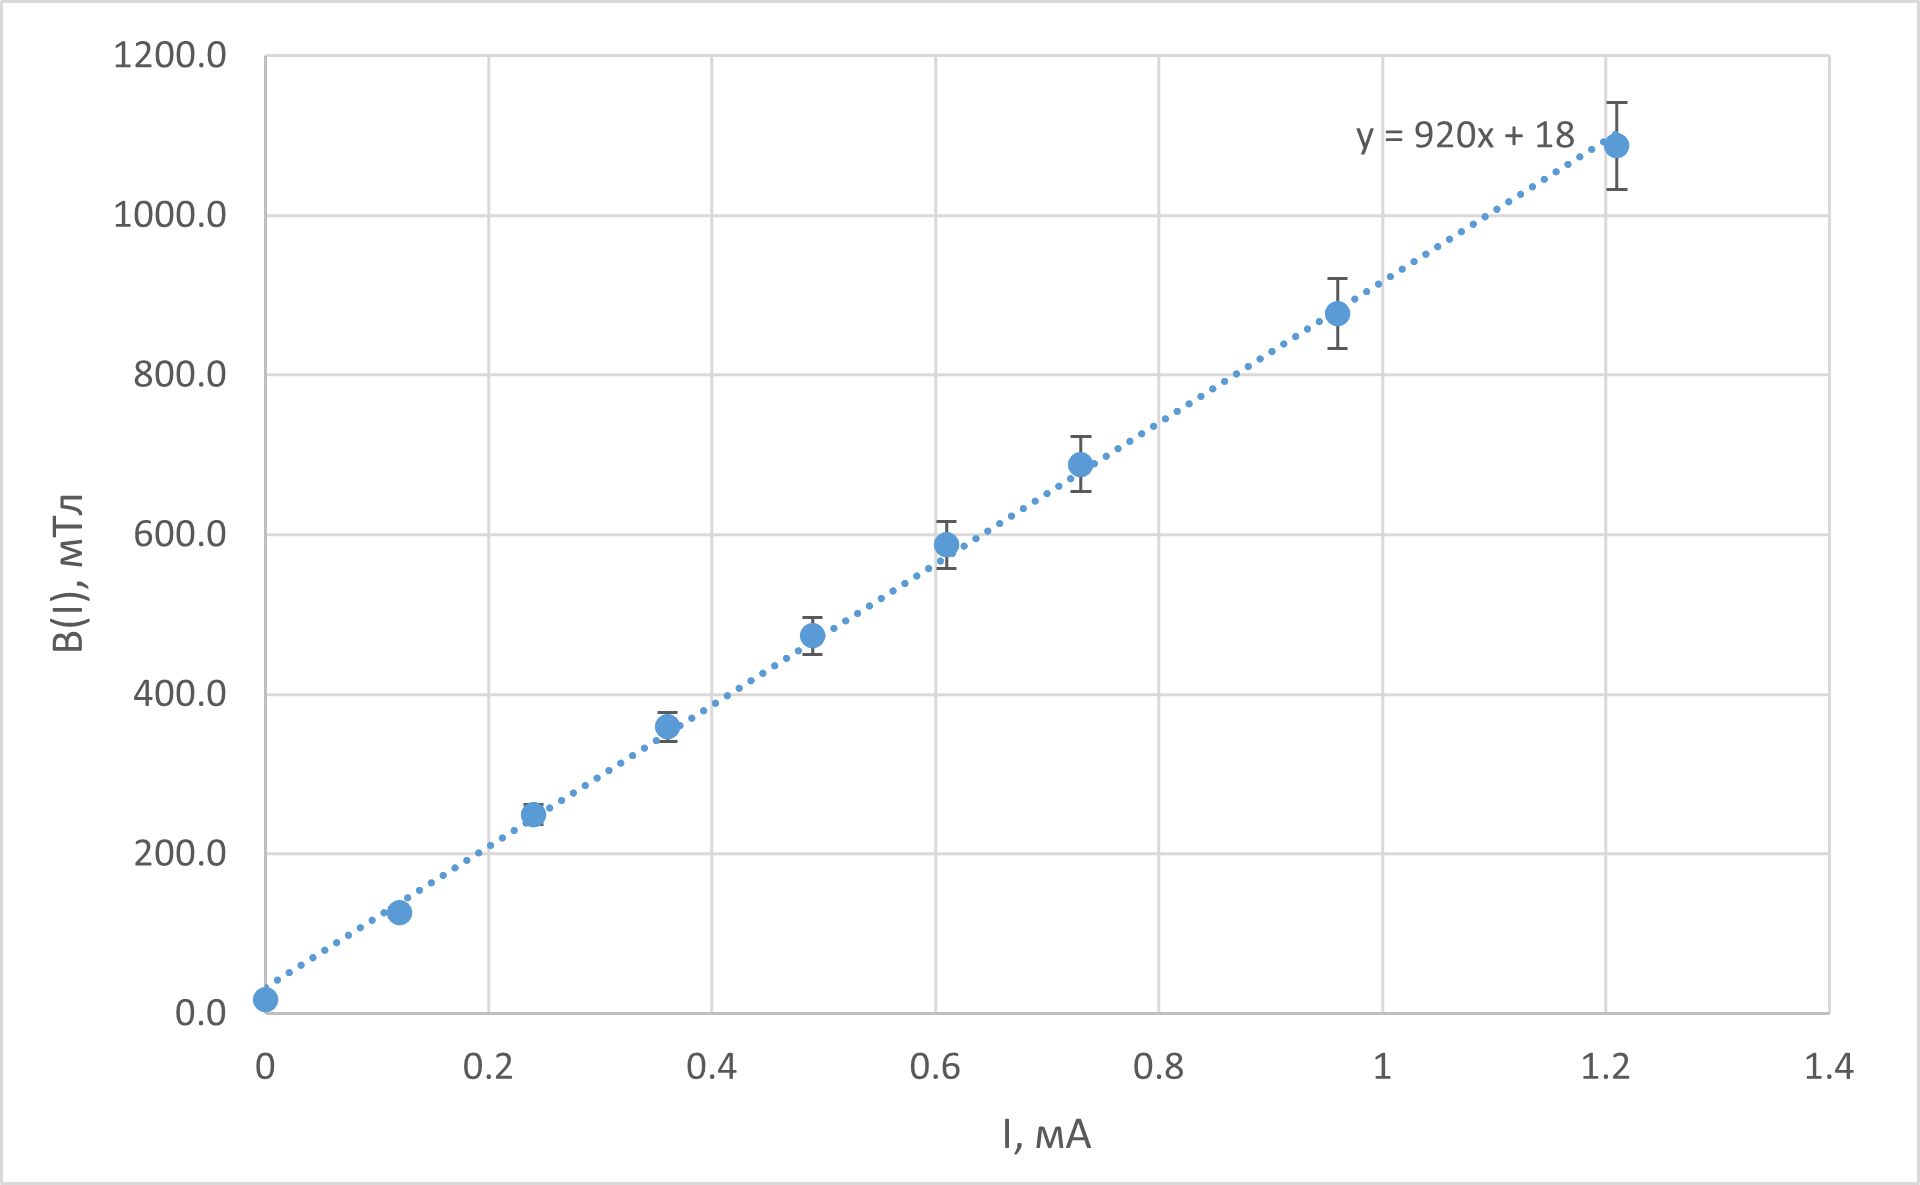
\includegraphics[width=0.9\textwidth]{pictures/калибр.png}
    \caption{Калибровочная прямая для электромагнита}
\end{figure} 

Методом Хи-квадрат найдем коэффциенты полученной прямой:

$$
    B(I) = 920 \cdot I + 18.0 \ (\text{мТл})
$$

\begin{itemize}
    \item $a = \left( 920\pm 9 \right)$ мTл/мA, \ $\varepsilon = 1.0$ \% 
    \item $b = \left( 18.0\pm 0.5 \right)$ мТл, \ $\varepsilon = 2.7$ \% 
\end{itemize}


\subsection{Зависимость k(B)}
Проведём измерение ЭДС Холла. Снимем зависимость напряжения $U_{34}$ от тока через обмотки магнита (с учётом $U_0$ при $I_M = 0$). Выполним серию экспериментов для различных токов через образец $I$ (от 0.3 до 1 мА). Построим на одном графике семейство прямых c k:
    
$$
   k = \frac{dU_{34}}{dB}
$$

Для построения графика будем пользоваться таблицей, связывающей ток в электромагните с магнитной индукцией в нем:

% Please add the following required packages to your document preamble:
% \usepackage{multirow}
% \usepackage[table,xcdraw]{xcolor}
% Beamer presentation requires \usepackage{colortbl} instead of \usepackage[table,xcdraw]{xcolor}
\begin{table}[H]
\centering
\caption{Зависимость индукции магнитного поля от тока в электромагните}
\label{t2}
\begin{tabular}{|c|c|c|c|}
\hline
\rowcolor[HTML]{A9D08E} 
I, мА & B, мТл & $\sigma_B$, мТл      & $\varepsilon$ \\ \hline
0    & 18     &                      & 8.0\%         \\ \cline{1-2} \cline{4-4} 
0.1  & 110    &                      & 8.4\%         \\ \cline{1-2} \cline{4-4} 
0.2  & 202    &                      & 4.6\%         \\ \cline{1-2} \cline{4-4} 
0.3  & 294    &                      & 3.1\%         \\ \cline{1-2} \cline{4-4} 
0.4  & 386    &                      & 2.4\%         \\ \cline{1-2} \cline{4-4} 
0.5  & 478    &                      & 1.9\%         \\ \cline{1-2} \cline{4-4} 
0.6  & 570    &                      & 1.6\%         \\ \cline{1-2} \cline{4-4} 
0.7  & 662    &                      & 1.4\%         \\ \cline{1-2} \cline{4-4} 
0.8  & 754    &                      & 1.2\%         \\ \cline{1-2} \cline{4-4} 
0.9  & 846    &                      & 1.1\%         \\ \cline{1-2} \cline{4-4} 
1    & 938    &                      & 1.0\%         \\ \cline{1-2} \cline{4-4} 
1.1  & 1030   &                      & 0.9\%         \\ \cline{1-2} \cline{4-4} 
1.2  & 1122   & \multirow{-13}{*}{9} & 0.8\%         \\ \hline
\end{tabular}
\end{table}

\begin{figure}[H]
    \centering
    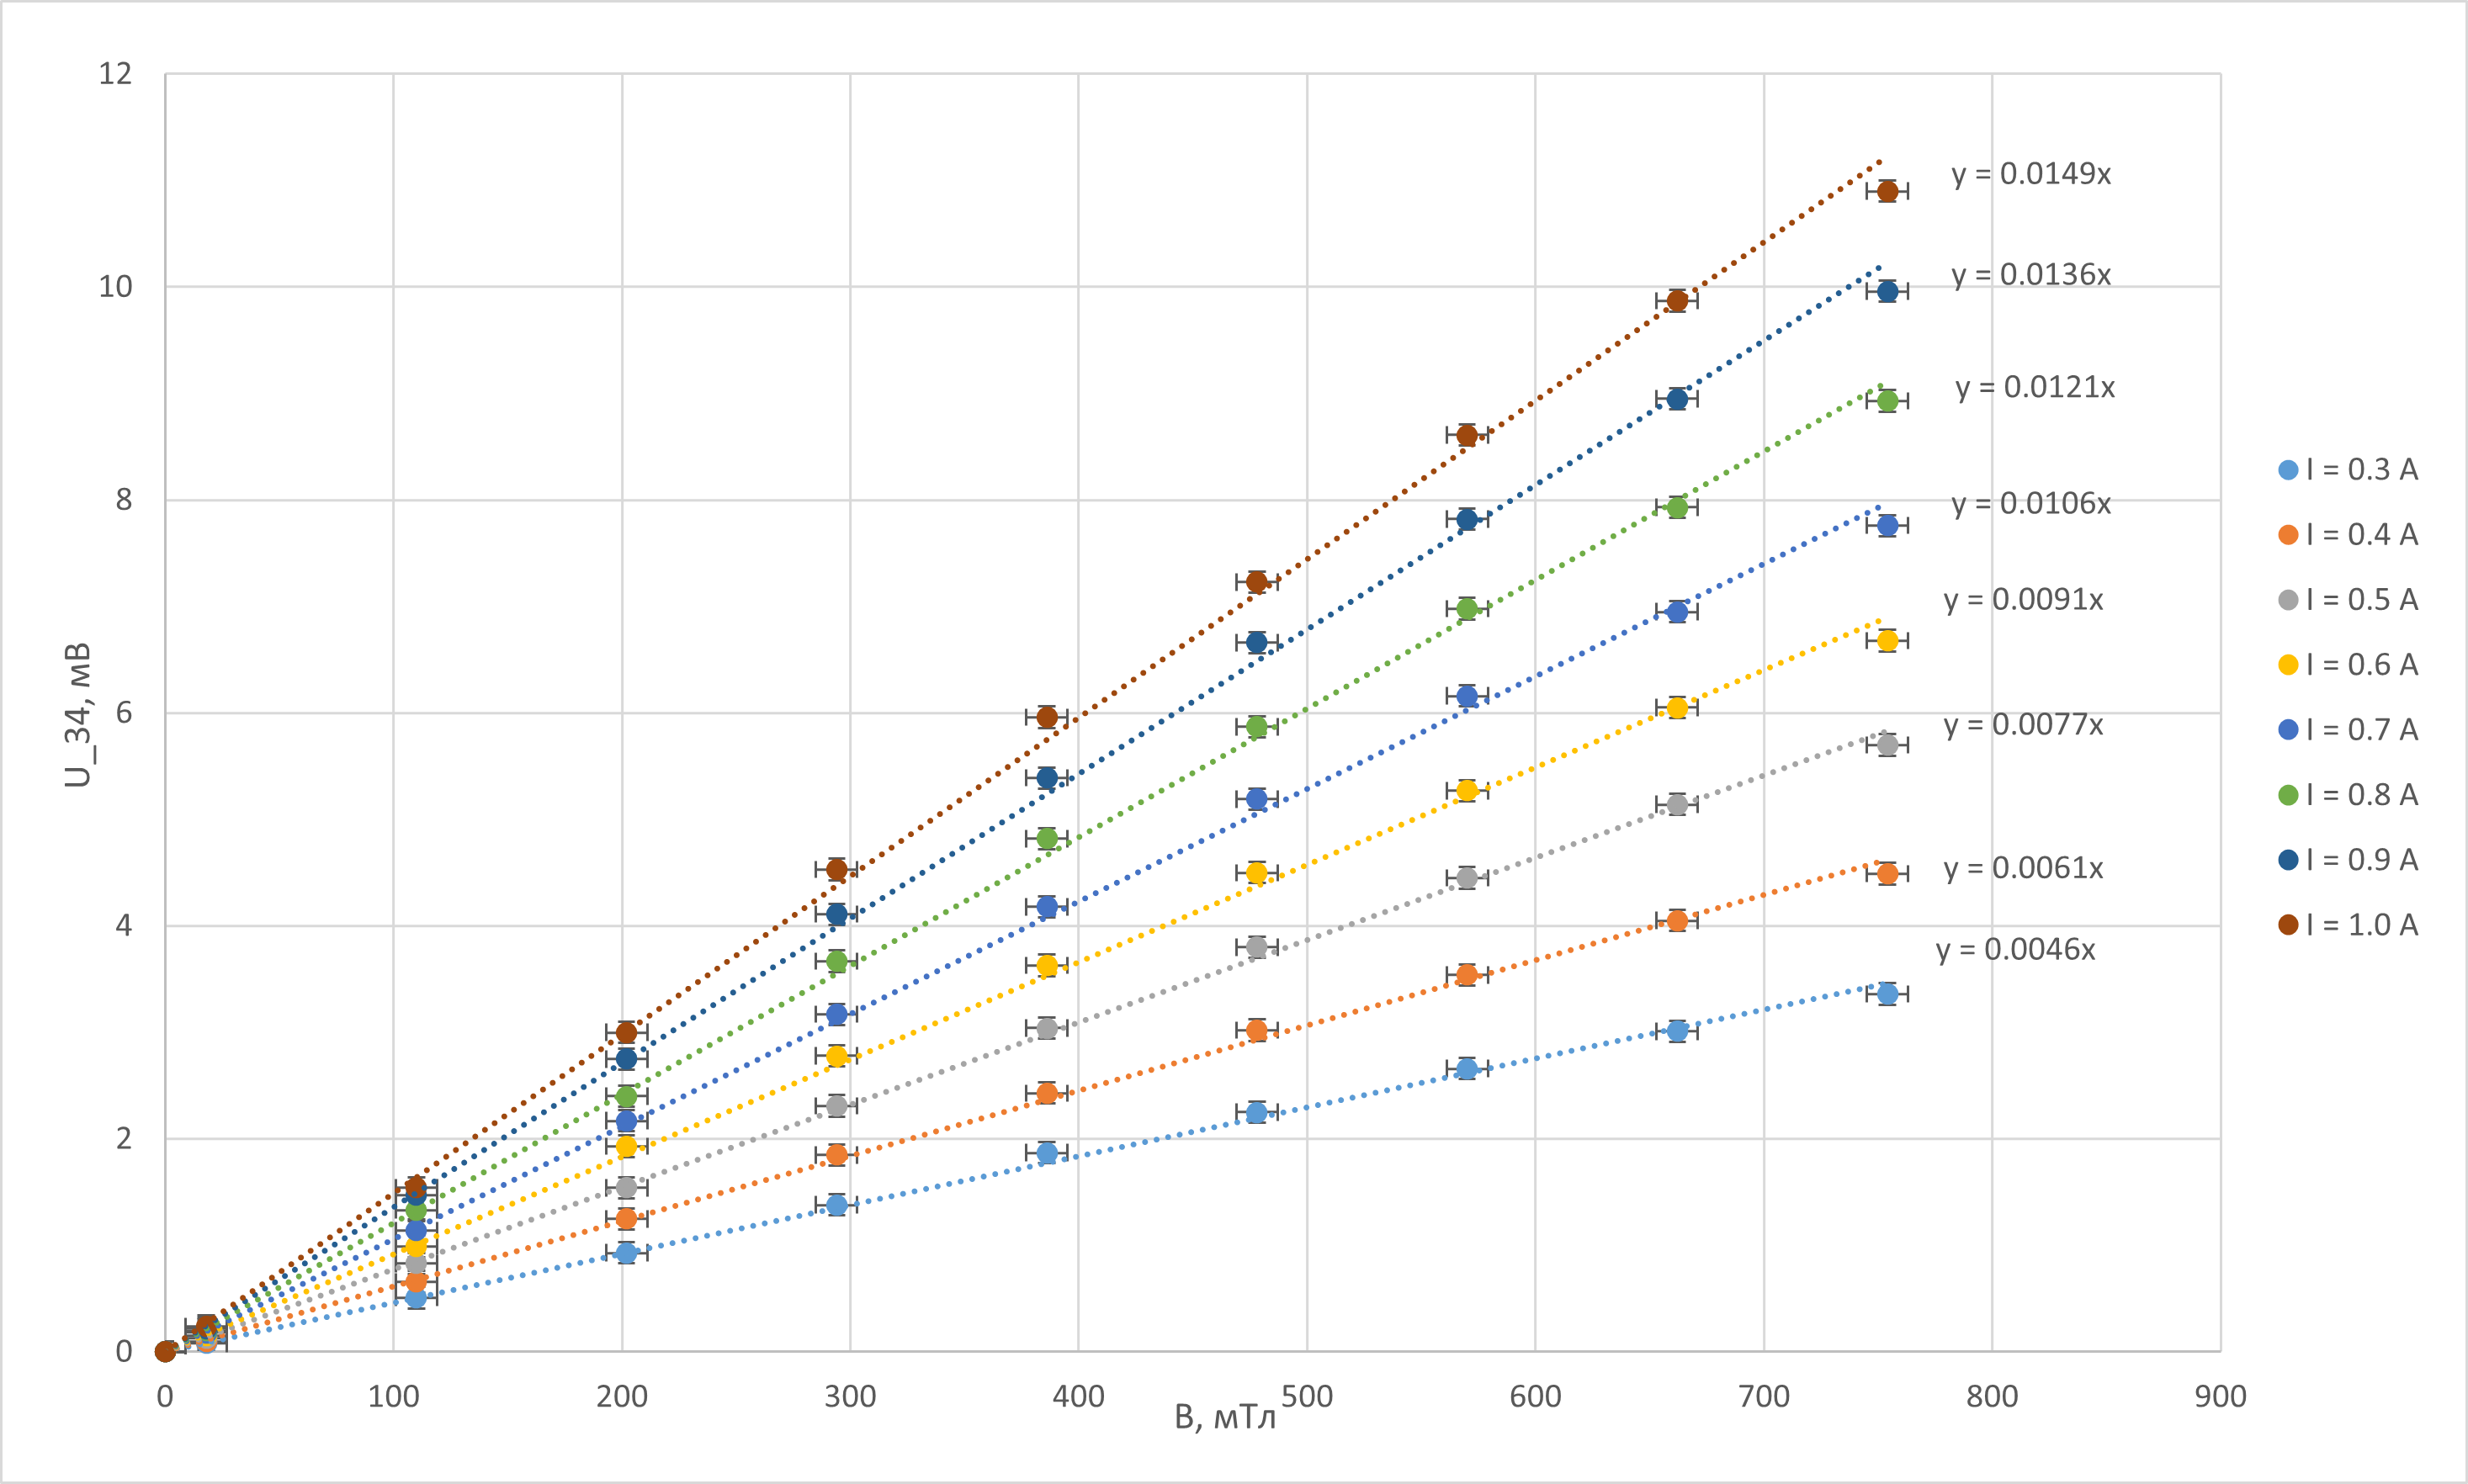
\includegraphics[width=1\textwidth]{pictures/все.png}
    \caption{Зависимость ЭДС Холла U от магнитного поля B при различных значениях тока через образец}
\end{figure} 

\subsection{Постоянная Холла}

Построим график зависимости K(I) по данным из таблицы:

% Please add the following required packages to your document preamble:
% \usepackage[table,xcdraw]{xcolor}
% Beamer presentation requires \usepackage{colortbl} instead of \usepackage[table,xcdraw]{xcolor}
\begin{table}[H]
\centering
\caption{Производная dU/dB = K при разных значениях тока в образце}
\label{t3}
\begin{tabular}{|c|c|c|c|}
\hline
\rowcolor[HTML]{A9D08E} 
I, мА & K, мкВ/мТл & $\sigma_K$,   мкВ/мТл & $\varepsilon$ \\ \hline
0.3  & 4.59       & 0.04                  & 1\%           \\ \hline
0.4  & 6.13       & 0.05                  & 1\%           \\ \hline
0.5  & 7.74       & 0.05                  & 1\%           \\ \hline
0.6  & 9.15       & 0.07                  & 1\%           \\ \hline
0.7  & 10.58      & 0.08                  & 1\%           \\ \hline
0.8  & 12.08      & 0.08                  & 1\%           \\ \hline
0.9  & 13.57      & 0.10                  & 1\%           \\ \hline
1    & 14.89      & 0.11                  & 1\%           \\ \hline
\end{tabular}
\end{table}

\begin{figure}[H]
    \centering
    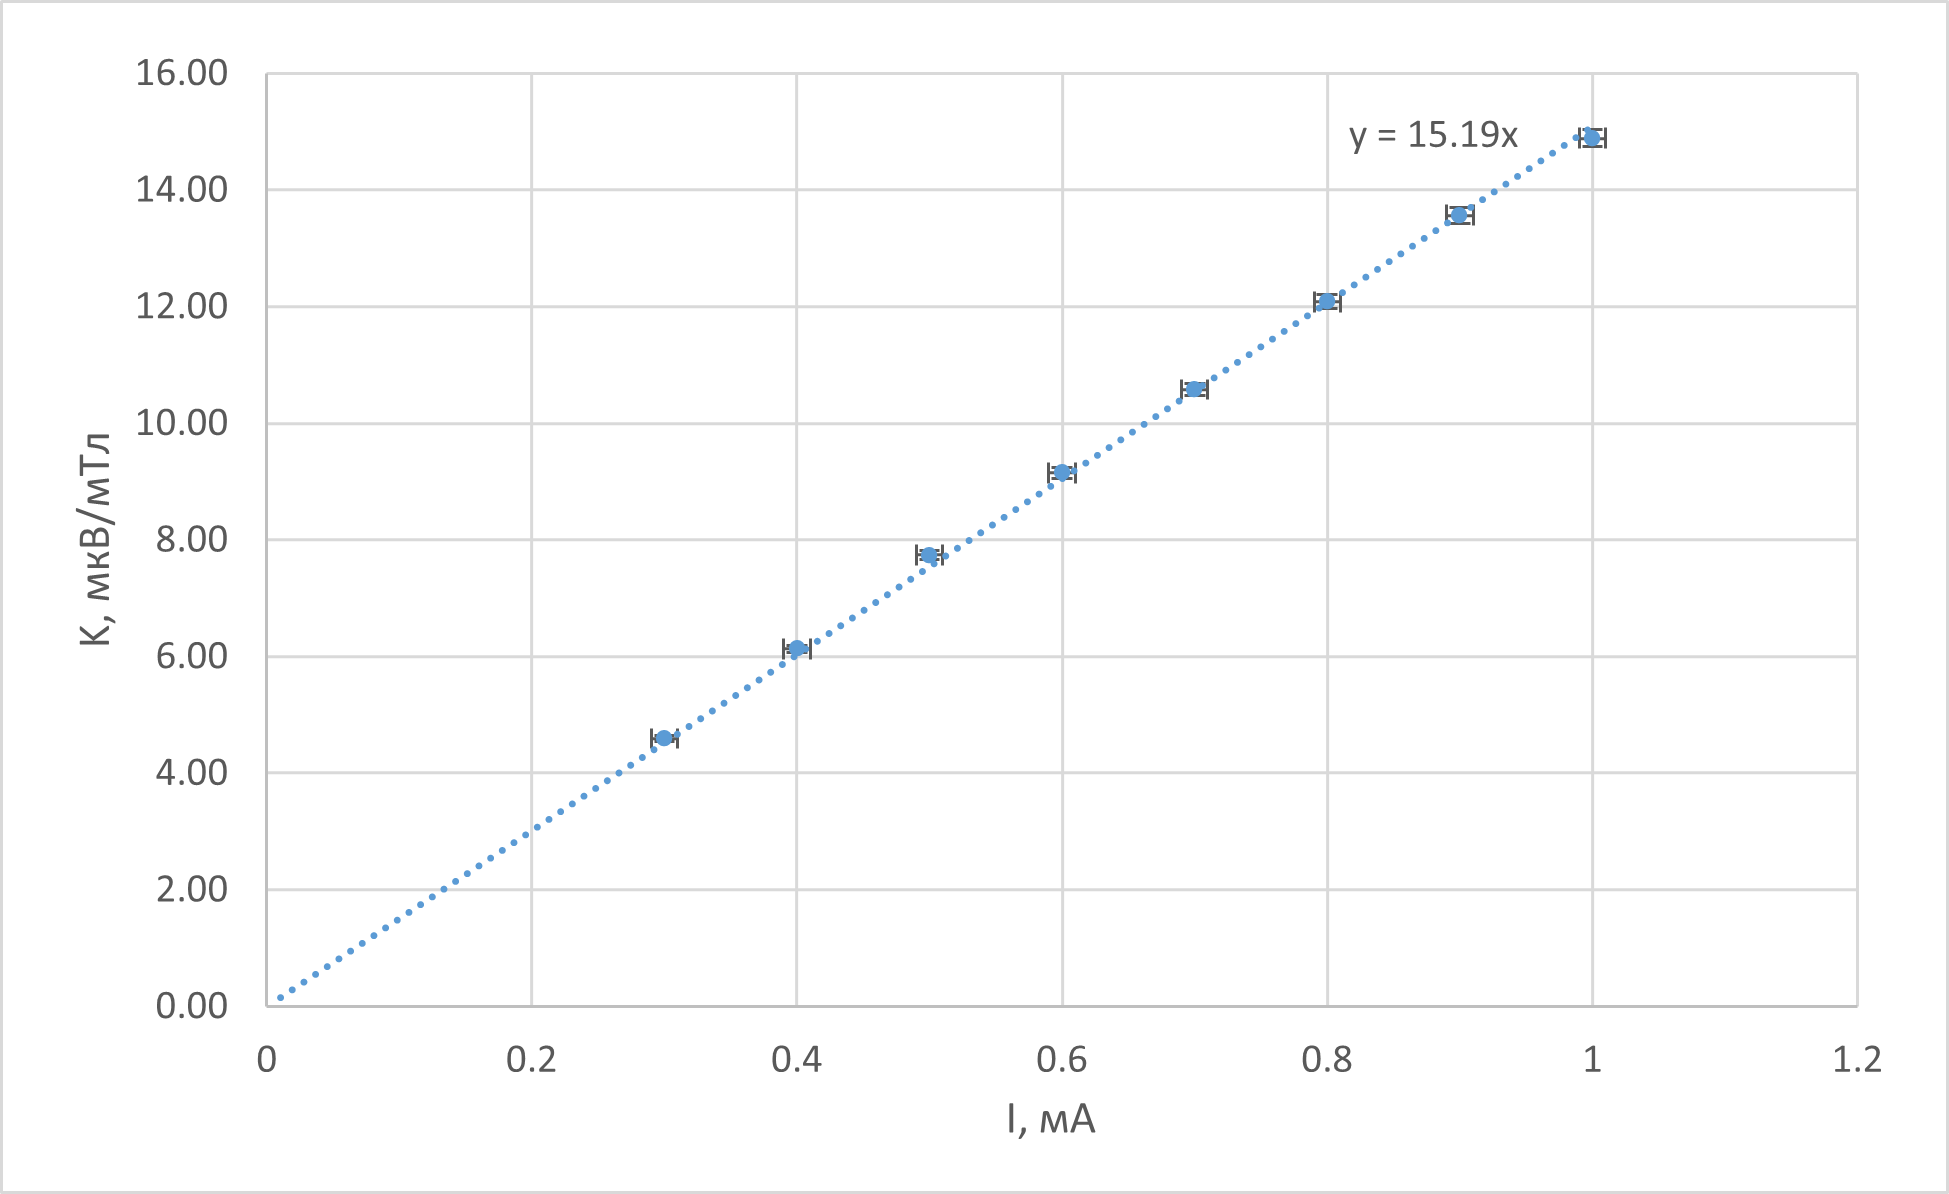
\includegraphics[width=1\textwidth]{pictures/K.png}
    \caption{График зависимости K = dU/dB от тока через образец}
\end{figure} 

Из него найдем коэффициент наклона, равный dK/dI:

$$
    \frac{dK}{dI} = \frac{R_x}{a}= (15.19
 \pm 0.07)  \ \frac{\text{В}}{\text{Тл*А}} \ (0.4 \%)
$$

Далее вычислим постоянную Холла:

$$
    R_x = (3.038 \pm 0.014) \cdot 10^{-2}  \ \frac{\text{м}^3}{\text{Кл}} \ (0.4\%)
$$

\subsection{Остальные расчеты}

Вычислим концентрацию носителей заряда следующим образом:

$$
    n = \frac{1}{R_x \cdot e} = (2.06 \pm 0.01) \cdot 10^{20} \ \frac{1}{\text{м}^3} \ (0.2\%)
$$


Параметры установки: h = 2 мм, a = 8 мм, l = 15 мм.
$$
    U_{35} = 81.1 \ \text{мВ}
$$

Вычислим удельное сопротивление материала образца по формуле (13):

$$
    \sigma_0 = \frac{Il}{U_{35} a h} = (1.16 \pm 0.01) \cdot 10^{-5}\ \frac{\text{1}}{\text{Ом $\cdot$ м}} (1 \%)
$$

$$
    \rho_0 = \frac{1}{\sigma_0} = (86.5 \pm 0.09) \cdot 10^{3} \ \text{Ом $\cdot$ м} (1 \%)
$$

Вычислим подвижность носителей заряда:

$$
    \mu = \frac{\sigma_0}{qn} = (4.00 \pm 0.04) \cdot 10^{-3} \ \frac{\text{см}^2}{\text{В $\cdot$ c}} (1 \%)
$$

\subsection{Определение знака носителей заряда}

Из рисунка следует, что знак носителей заряда отрицательный. Если бы знак был положителен, то при исходных условиях мы бы пришли к явному противоречию.

\begin{figure}[H]
    \centering
    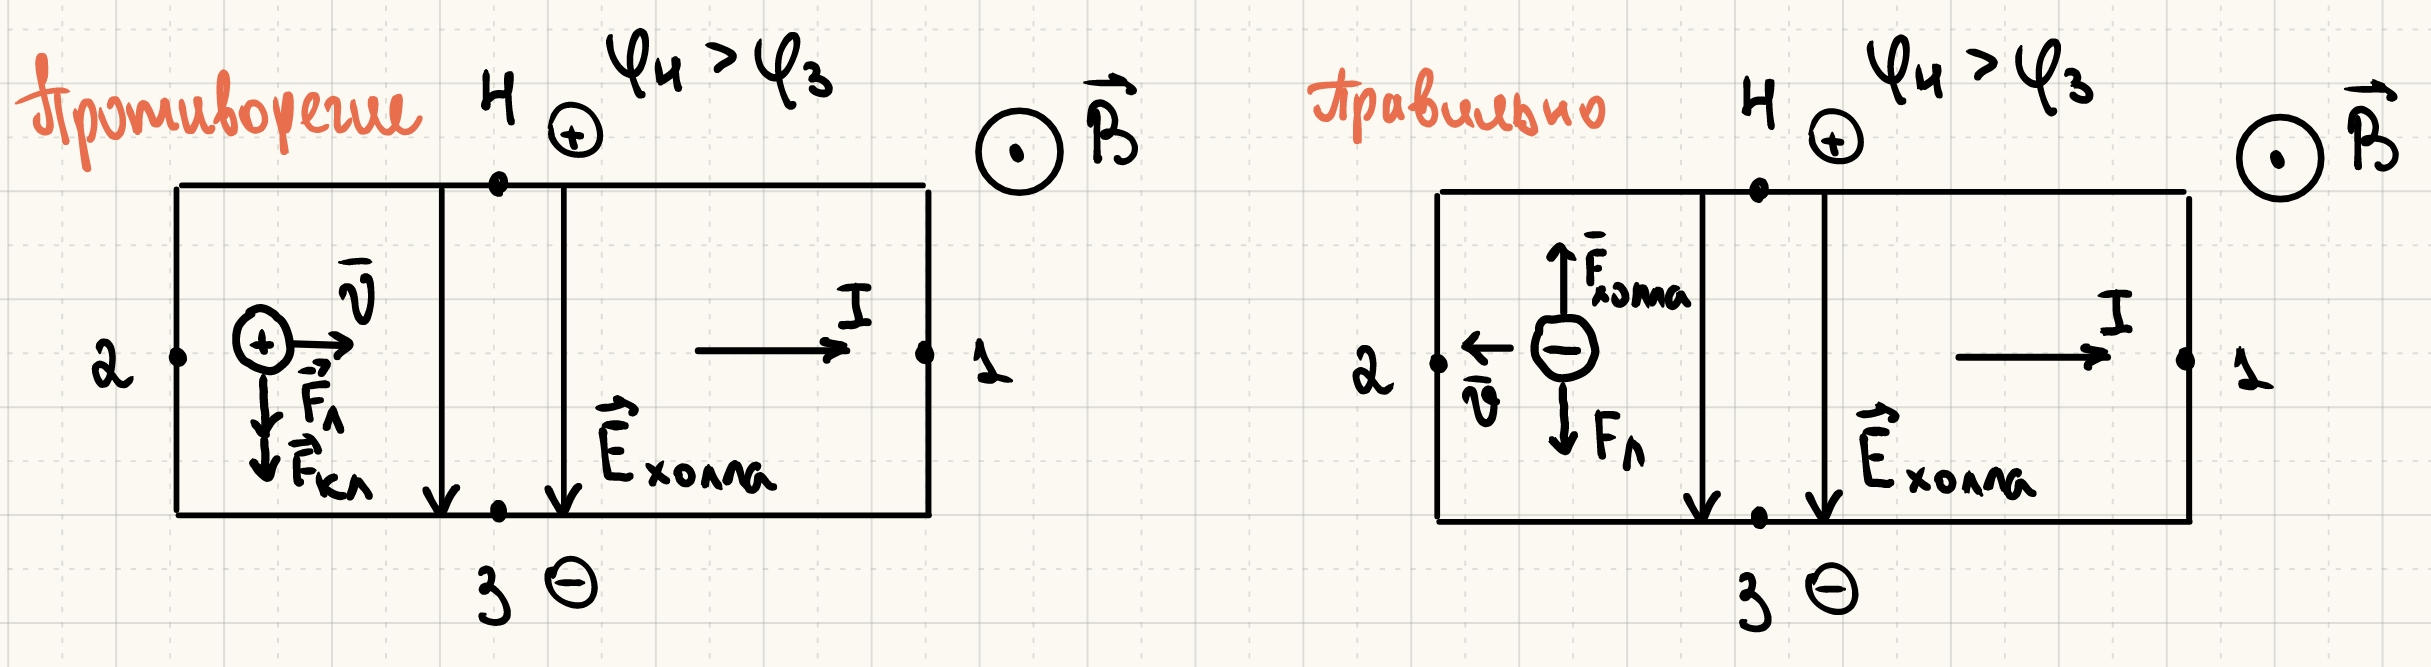
\includegraphics[width=1\textwidth]{pictures/LAST.jpg}
\end{figure} 


    

